\documentclass[12pt]{article}
%
\usepackage{makeidx}  % allows for indexgeneration
\usepackage{pslatex}
\usepackage{graphicx}
\usepackage{float}

% \makeatletter
% \newcommand{\rmnum}[1]{\romannumeral #1}
% \newcommand{\Rmnum}[1]{\expandafter\@slowromancap\romannumeral #1@}
% \makeatother
%
\begin{document}
%
%\frontmatter          % for the preliminaries

%\mainmatter              % start of the contributions
%
\title{Mechanisms for Generating Mosaic Structures of Segmental Duplications}
%
%\titlerunning{CAP project}  
%\author{Yu Lin}
%\institute{}

%
\maketitle              

\section{Introduction}

Genome-scale evolutionary events include genome rearrangements, duplications and deletions. 
Genome rearrangements, which shuffle gene orders and change the gene orientations, 
includes inversions, transpositions, translocations, fusions, and fissions. 

In this paper, we focus on special type of duplications called segmental duplications. 
Segmental duplications are segments of DNA (typically range at least 1kb in length), 
occur at more than one site within the genome, and typically share a high level of sequence identity ($>90\%$)~\cite{eichler2001}. 
Segmental duplications have long been recognized as driving forces of evolution~\cite{bailey2006primate}. 
For example, segmental duplications in human genomes are hotspots 
for nonallelic homologous recombination, copy-number variations, genes and transcripts innovations~\cite{jiang2007ancestral}. 
Segmental duplications in human genomes generally form mosaic structures combining or juxtaposing original segments 
that range from 1kb to 200 kb from disparate regions of the genome~\cite{samonte2002segmental}. 
Subsequent duplications duplicate portions of mosaic structures to other regions of the genome---create additional copies of the initial segments, 
in which the order of the duplicated segments is generally preserved~\cite{bailey2002human}. 
Pevzner \emph{et al.} proposed to use A-Bruijn graphs to represent repeats and sub-repeats of mosaic structures in a genome ~\cite{pevzner2004}. 
Jiang \emph{et al.} applied A-Bruijn graphs to study ancestral reconstruction of segmental duplications that emerged within the last 40 million years of human genome evolution,  
based on a collection of 28,856 pairwise alignments (with length $>$1kbp and sequence identity $>$90\%)~\cite{jiang2007ancestral}.

The formation of mosaic structures of segmental duplications seems to involve complex rearrangements and duplications, but the mechanism behind it is still unclear.
Recent studies on genomic disorders from clinical chromosomal microarray analysis revealed similar complex patterns of rearrangements and duplications ~\cite{lee2007dna,liu2011chromosome}. 
The analyses of sequences at breakpoint junctions by array comparative genomic hybridization (aCHG)~\cite{pinkel2005array}, 
led to the proposal of a replication based mechanism, 
the Fork Stalling and Template Switching (FoSTeS) model~\cite{lee2007dna} (inspired by a similar mechanism proposed for amplification in E. coli \cite{slack2006mechanism}) 
and the Microhomology Mediate Break-Induced Replication (MMBIR) model~\cite{hastings2009microhomology}. 
According to this mechanism, during DNA replication, 
long-distance template-switching occurs between replication forks in physical proximity (not necessary adjacent in primary sequences) through the microhomology.
Depending on whether the position and orientation of the new fork was invaded and copied, and the direction of fork progression, 
template-switching results in a duplication, deletion, inversion or translation~\cite{hastings2009microhomology}. 
This procedure of long-distance template-switching could occur multiple times in series, 
due to the poor processivity of the involved DNA polymerase, causing the complex rearrangements and duplications~\cite{gu2008mechanisms}.

     
We hypothesize that the formation of mosaic structures of segmental duplications involves a replication based mechanism for the following reasons.
\begin{itemize}
\item The replication based mechanism can account for complex rearrangements and duplications from the observed clinical genomic data, 
including juxtaposing of distantly distributed segments, a phenomenon resembling mosaic structures of segmental duplications.
\item The original segments are usually 1kb to 200 kb away from the duplicated segments in the mosaic structures~\cite{samonte2002segmental}, 
and such distances are below the long distances in the observed template-switchings (e.g., 120kb to 550kb ~\cite{gu2008mechanisms}).
\end{itemize}

We will use de Bruijn graphs built from genome sequences to check whether the formation of mosaic structures of segmental duplications involves a replication based mechanism. 
\begin{enumerate}
\item For human genomes, we first need to deal with the high-multiplicity mobile elements (e.g. SINE and LINE repeats). 
 The most common SINE repeats in primates are called Alu elements, each approximately 260 base pairs long. 
 The human genome contains estimated over one million Alu elements---about $11\%$ of the genome~\cite{lander2001}, 
 and about half a million LINE repeats---about $17\%$ of the genome~\cite{cordaux2009}. 
 We could mask all known the Alu elements and LINE repeats, by replacing them with random sequences of same lengths, 
 but still record their position information for later analysis, 
 since these high-multiplicity mobile elements may trigger complex long-distance template-switchings 
 and serve as footprints at the breakpoint junctions~\cite{carvalho2011inverted}. For E. coli genomes, we may not need this preprocess.
 \item We build a de Bruijn graph from the input genome, by transforming that genome into perfect sequencing reads of (k+1)-mer (overlapping and uniform coverage).
 Note that this de Bruijn graph can only ``glue'' all perfect repeats without any gaps and mismatches. 
 We could handle imperfect repeats by the techniques in SPAdes~\cite{spades} (e.g., error corrections in reads and simplification of A-Bruijn graphs). 
 Note that we may first focus on near-perfect repeats.
 \item We find out all the candidates for the mosaic structures of segmental duplications in the input genomes. 
 A candidate is a continuous region that duplicates and juxtaposes distantly distributed segments on the same arm of the chromosome.
 Figure~\ref{candidate} illustrates an example of a candidate for a mosaic structure of segmental duplications in the de Bruijn graph. 
 Note that these duplicated segments are linked by edges of approximate length ~k (in terms of the number of k-mers, see brown edges in Figure~\ref{candidate}).
\begin{figure}[H]
\begin{center}
\includegraphics[width=1.0\textwidth]{mosaic.eps}
\caption{An example for a mosaic structure of segmental duplications and the corresponding part of the de Bruijn graph}
\label{candidate}
\end{center}
\end{figure}

\item For each candidate mosaic structure, we retrieve the sequence information from the de Bruijn graph, 
and check whether there are microhomology~\cite{hastings2009microhomology} or novel sequence insertions from neighboring regions at the breakpoint junctions~\cite{liu2011chromosome}.
Note that microhomology of $m$ bps at the breakpoint junctions may result in the $(k-m)$-length edges linking adjacent segments in a mosaic structure.
\end{enumerate}


\section{Followup: the Breakpoint Graph and the Colored de Bruijn Graph}

Assume that a genome is a set of strings. Given genomes $A$ and $B$, we classify ($k$+$1$)-mers in the genomes into 3 classes: 
$A$(occur only in $A$), $B$(occur only in $B$) and AB(occur in both $A$ and $B$). 

\subsection{the Breakpoint Graph}
The breakpoint graph is a data structure first introduced by Bafna and Pevzner to study the inversion distance~\cite{bafna1993}, 
which has formed the basis for much algorithmic research on rearrangements over the last twenty years. 
Alekseyev and Pevzner extened the pairwise breakpoint graphs~\cite{bafna1993} to the multiple breakpoint graphs 
to overcome some limitations in the study of ancestral genome reconstructions~\cite{alekseyev2009}.
However, it is difficult to incorporate segmental duplications into breakpoint graphs, 
since breakpoint graphs are usually defined on genomes with equal gene content and no duplicates.

Given a set of strings $S$, the breakpoint graph $BP(S)$ is defined as follows.
\begin{itemize}
\item Each $k$-mer in the strings is a directed edge with two vertices, $u$ as its start and $v$ as its end,
and each $k$+$1$-mer in the strings is an undirected edge which connects the end of its prefix $k$-mer and the start of its suffix $k$-mer.
\item Identically labeled edges ($k$-mers) are glued together.
\end{itemize}

The colored breakpoint graph is simply coloring the edges of the breakpoint graph $BP(A \bigcup B)$ into 3 colors: $A$(red), $B$(Blue) and $AB$ (purple).
There are two kinds of non-branching and unicolored paths in the colored breakpoint graphs. 
Type $I$ paths are from an end of a $k$-mer to a start of another $k$-mer, and type $II$ paths are from a start of a $k$-mer to an end of another $k$-mer.  
We can condense the colored breakpoint graphs by replacing type $I$ paths with undirected colored edges, 
and type $II$ paths with directed colored edges (e.g., see Figure~\ref{transposition} (d) and (e)). 
Note that the traditional pairwise breakpoint graphs~\cite{bafna1993} correspond to the condensed (colored) breakpoint graphs (e.g., see Figure~\ref{transposition} (e)).

\subsection{the Colored de Bruijn Graph}
The de Bruijn graph is a data structure first brought to bioinformatics by Pevzner as a method to assemble k-mers
generated by sequencing by hybridization~\cite{pevzner1989}, and is later used in sequence assembly~\cite{idury1995,pevzner2001eulerian}.

Given a set of strings $S$, the de Bruijn graph $DB(S)$ is defined as follows.
\begin{itemize}
\item Each $k$-mer in the strings is a vertex, 
and each $k$+$1$-mer is a directed edge from its prefix $k$-mer to its suffix $k$-mer.
\item Identically labeled vertices ($k$-mers) are glued together.
\end{itemize}
A non-branching paths in de Bruijn graph can be replaced by a directed edge of which the direction is from its directed edges ($k$+$1$-mers). 
The condensed de Bruijn graph replaces all non-branching paths by single edges.

The colored de Bruijn graph $G(A,B)$ is simply coloring the edges of the de Bruijn graph $DB(A \bigcup B)$ into 3 colors: $A$(red), $B$(blue) and $AB$ (purple). 
We can condense the colored de Bruijn graph by replacing all non-branching and unicolored paths by directed colored edges (e.g., see Figure~\ref{transposition} (b) and (c)).

The bi-directed de Bruijn graphs~\cite{medvedev2007} can be viewed as gluing reverse complement k-mers (vertices) in the de Bruijn graph. 
This notation can also easily extended to the colored de Bruijn graphs and their condensed forms (e.g., see Figure~\ref{inversion2} (b) and (c)).

\newpage{}

\subsection{Colored de Bruijn Graph v.s. Breakpoint Graph}
Figure~\ref{transposition} illustrates an example of a transposition. Note only one strand is shown in the figure.
A cycle in an edge-colored graph is called alternating if the colors of every two consecutive edges of this cycle are distinct. 
Figure~\ref{transposition} (c) and (e) contain alternating cycles.
\begin{figure}[H]
\begin{center}
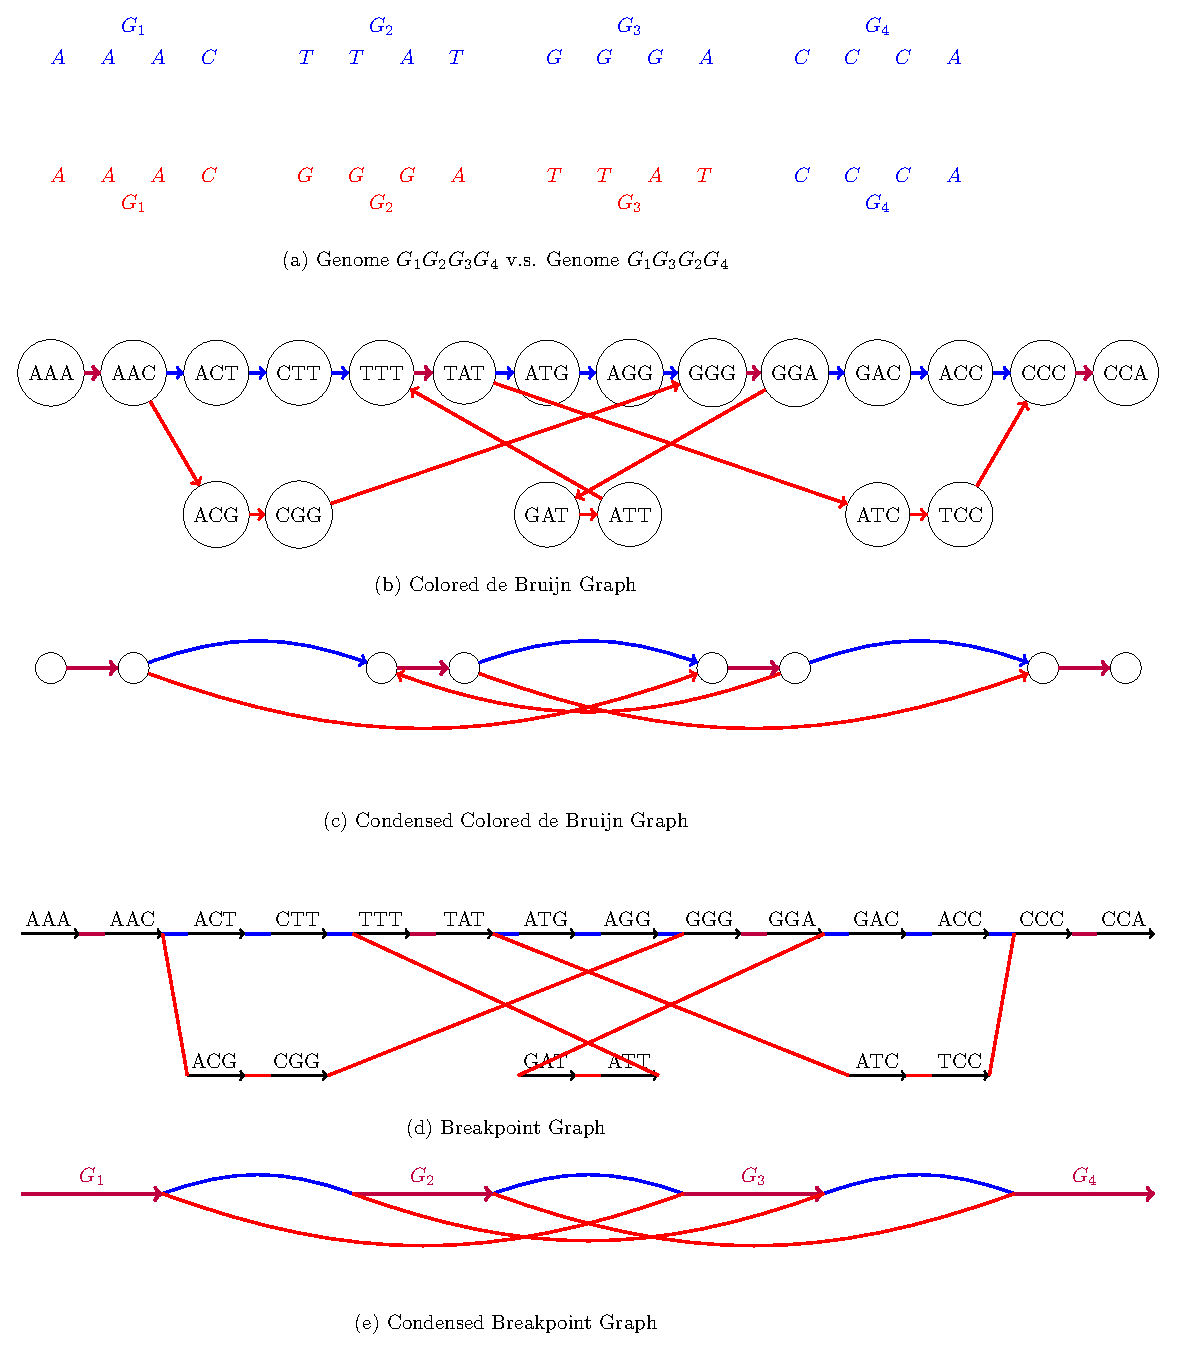
\includegraphics[width=0.9\textwidth]{transposition_new.eps}
\caption{A toy example of a transposition.}
\label{transposition}
\end{center}
\end{figure}

\newpage{}

Figure~\ref{inversion} illustrates an example of an inversion on the de Bruijn graph of both strands.
Note the both strands are used to the formulate of alternating cycles.
\begin{figure}[H]
\begin{center}
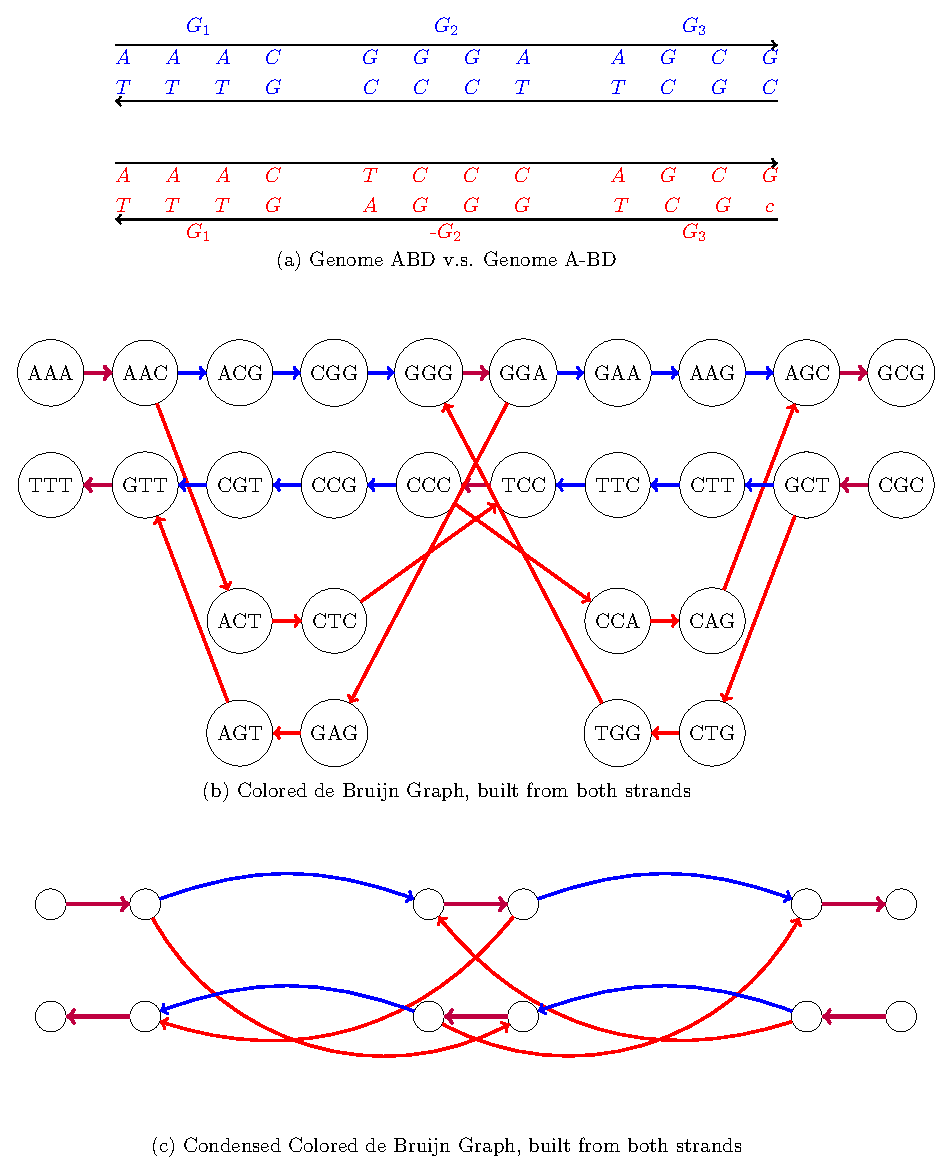
\includegraphics[width=0.85\textwidth]{inversion.eps}
\caption{A toy example of an inversion on the de Bruijn graph of both strands.}
\label{inversion}
\end{center}
\end{figure}

\newpage{}


Figure~\ref{inversion2} illustrates the same example of an inversion by gluing each k-mer with its reverse complement as in the bi-directed de Bruijn graph~\cite{medvedev2007}.
\begin{figure}[H]
\begin{center}
\includegraphics[width=0.9\textwidth]{inversion_glue.eps}
\caption{A toy example of an inversion on the bidirected de Bruijn graph.}
\label{inversion2}
\end{center}
\end{figure}

The above toy examples show that the simplified colored de Bruijn graph is very similar to the corresponding breakpoint graph. 
But the following properties are worth noticing.
\begin{itemize}
 \item Rearrangements create edges of center size in the condensed colored de Bruijn graph. 
 For example, each read or blue edge caused by rearrangements in alternating cycles should have length around k (in terms of the number of (k+1)-mer edges).
 \item Assume there is no large duplications and losses, for each alternating cycle caused by rearrangements in the condensed colored de Bruijn graph, 
 the sum of lengths of blue edges and that of red edges should have similar values.
\end{itemize}



\subsection{Why Colored de Bruijn Graphs?}
\begin{itemize}
 \item Extended model for both genome rearrangements, duplications and deletions. 
 \item Direct use of the sequence information
 \item Convenient incorporation of reference genomes for comparative study (multi-colored de Bruijn graph)
 \item Accurate prediction of boundaries of the evolutionary events (thanks to the high resolution)
 \item Detection of interesting genomic patterns/features (e.g. the mosaic structure in segmental duplications)
\end{itemize}

% \subsection{Possible difficulties with Colored de Bruijn Graphs}
% \begin{itemize}
% \item Mutations, small insertions and deletions\\
%  Please refer to the extensive discussions from Sergey on possible refinement strategies to overcome them.  
% \item Large repeats\\
%  The similar problem also occurs in the rearrangements with duplicates. When there are repeats, the cycle decomposition of the breakpoint graph is no longer unique. 
%  Better cycle decompositions are preferred, since they are corresponding to fewer number of evolutionary events between input genomes. 
%  We may apply greedy and matching-based algorithms to maximize the number of length-4 cycles~\cite{shao2012}. 
%  We could also make use of reference (outgroup) genomes to predict the relationships of these repeats (e.g., ancestral v.s. derived, contiguous v.s. independent). 
% \item Regions with nested rearrangements and duplications\\
%  We could define an overlap level on a region, to measure the number of overlapping/nesting evolutionary events on it. If the overlap level is too high, 
%  there is no easy way to recover those evolutionary events. 
%  If the overlap level is relatively low (which should be the case for most regions), we can enumerate all possible patterns in the Colored de Bruijn graph 
% and thus recover those events.
% \item Applications to biological datasets\\
% Many unexpected questions will appear when we start analyze biological datasets. 
% We could start from certain closely related species, where there are only a few known rearrangements or segmental duplications.
% We could try to map these known evolutionary events to the Colored de Bruijn graph constructed from sequence data, 
% and thus motivate ourselves to check to what extent we have made progress. 
% Such comparison may boost our confidence or reveal new challenges that we need to address in the future.
% 
% \end{itemize}
% 
% \section{A Case Study---E. coli}
% Sergey tested the current tool on the comparison between E. coli K-12 strain and other E. coli strains. 
% One candidate of a transposition is described in Figure~\ref{ecoli_transposition}.  
% \begin{figure}[H]
% \begin{center}
% 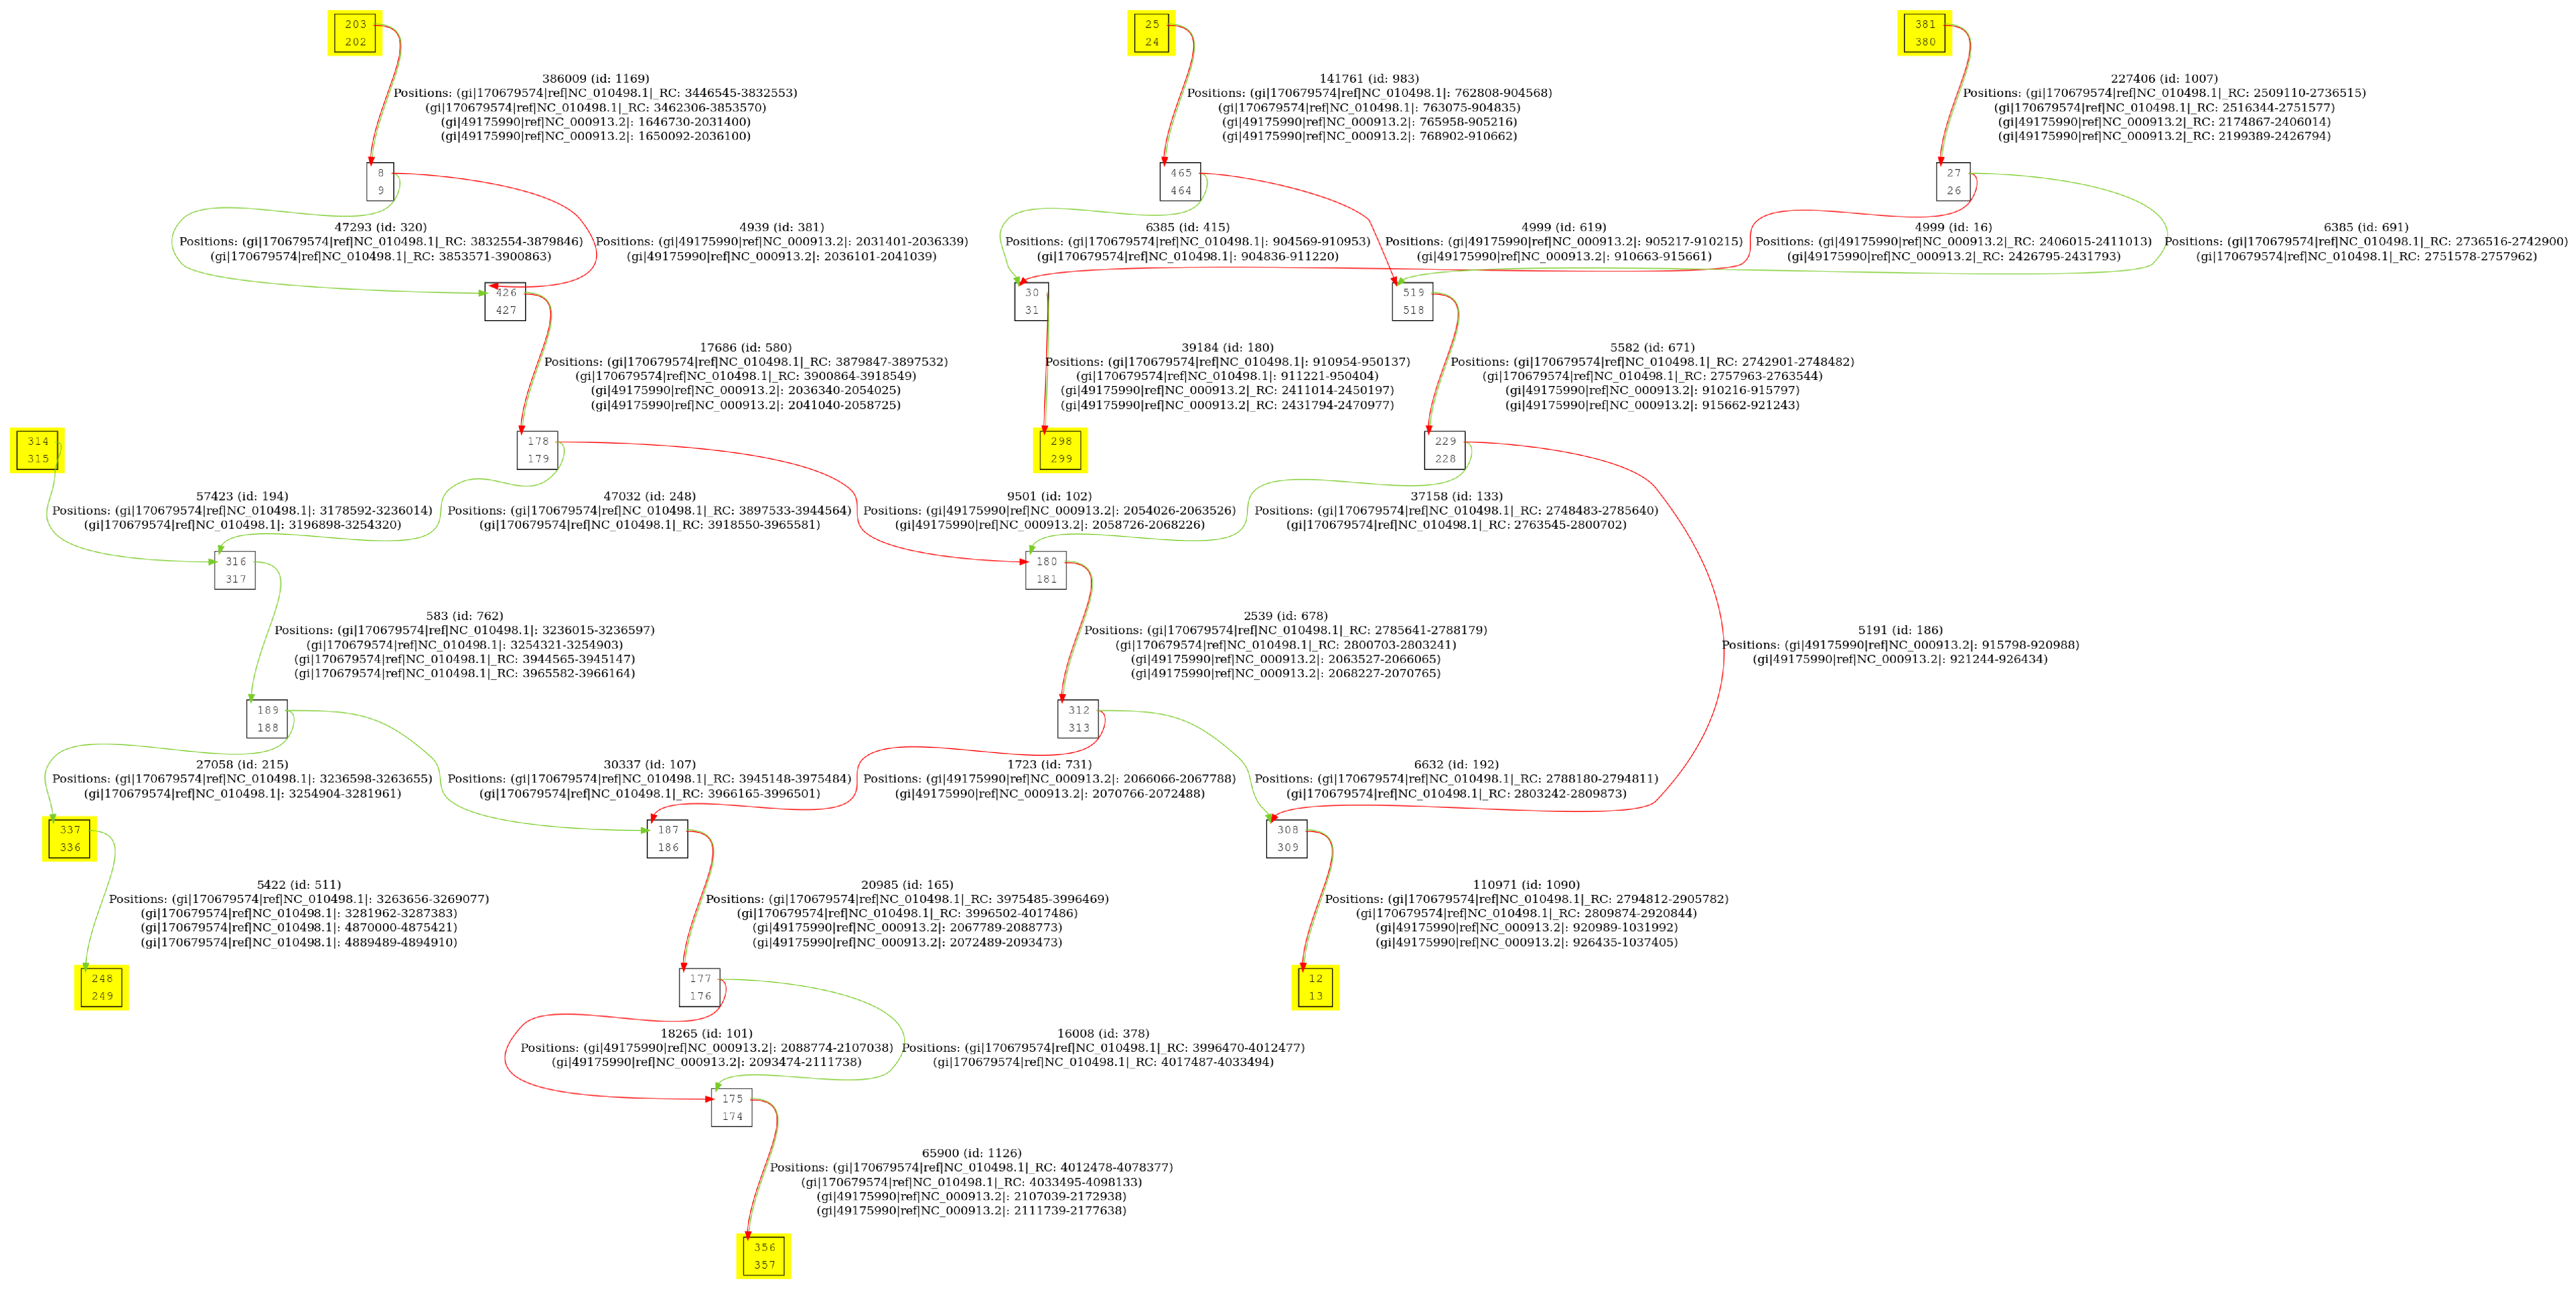
\includegraphics[width=\textwidth]{ecoli_transposition.eps}
% (a) the original colored de Bruijn graph\\
% ~~\\
% 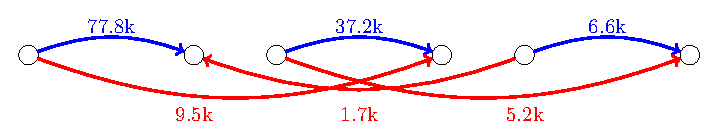
\includegraphics[width=\textwidth]{ecoli_transposition_new.eps}
% (b) a cycle in the simplified colored de Bruijn graph from the above graph 
% \caption{A candidate of a transposition in the colored de Bruijn graph from pairwise comparison of E. coli strains. 
% In both (a) and (b), each k-mer has 5001 nucleotides. The length of each edge, in terms of the number of (k+1)mer edges, is marked above or below that edge in (b).}
% \label{ecoli_transposition}
% \end{center}
% \end{figure}
% 
% Let us compare this case with the ideal case. 
% \begin{itemize}
%  \item In the ideal case, all edges in the simplified de Bruijn graph should have length around k, 
%  but in the above case, only 2 out of 6 edges have length around k=5001 (5.2k and 6.6k in Figure~\ref{ecoli_transposition}).
%  We may expect some deviations from the expected length of edges (=5001) in the simplified de Bruijn graph, 
%  but other lengths (1.7k, 9.5k, 37.2k and 77.8k) may not be explained by only local mutations and small indels. 
%  The 1.7k edge is much shorter than the expected length, which may be due to repeats in the blue genome.
%  Other larger lengths (9.5k, 37.2k and 77.8k) may be due to large duplication events.
%  \item In the ideal case, the sum of lengths of blue edges and that of red edges in the same cycle should have similar values, 
% but in the above case, these two values are (9.5+1.7+5.2=)16.4k and (77.8+37.2+6.6=)121.6k, which are very different!
% The blue genome is much longer than the red genome at the same perturbed region. 
% We may infer that there are some duplication events happened in the blue genome. 
% We need to introduce other reference strands into the comparison. 
% If the reference genomes at this interesting region can be clustered into two clusters, one with much shorter sequences and with the order as the red genome, 
% the other with much longer sequences and with the order as the blue genome, this may hint that this transposition is closed related to duplications (thus duplications may trigger rearrangements).
% \item In the ideal case, all edges in the simplified de Bruijn graph accurately mark the boundaries of rearrangement operations, since each edge has length around k.
% But in the above case, the boundaries of this potential transposition may be very difficult to be estimated. 
% We can again introduce reference genomes as in the study of comparative genomics. 
% By introducing reference genomes, 
% long edges in the original bi-colored de Bruijn graphs may be decomposed into shorter ones in multi-colored de Bruijn graphs.
% Those edges with length around k form candidates of marking accurate boundaries between synteny blocks,
% which may provide more information about the real evolutionary scenarios.
% \item Is it possible that this is an HGT (Horizontal Gene Transfer) instead of a transposition and what is the direction of this HGT? 
% HGT may introduce asymmetry in the sum of lengths of blue edges and that of red edges in the same cycle, as well as variations in lengths of the edges. 
% One possible task is to distinguish an HGT from a transpositions by introducing reference genomes and the phylogeny of these genomes. 
% We need to figure out whether the transposed block is from its own genome or from some other genomes. 
% For example, in an HGT, some siblings of the genome which receives the transposed block do not have that block in their genomes; 
% in a transposition, all the siblings of both genomes typically have the transposed block.
% 
% \end{itemize}
% 
% More cases are needed! (Sergey is now working on masking repeats within the same strand, and collecting more cases that may correspond to potential rearrangement operations.)

% \section{Address biological challenges---segmental duplications and rearrangements in primate genomes}
% \begin{itemize}
%  \item {\bf Can we find segmental duplications and mosaic structures directly from the de Bruijn graph?}\\
%  The current building blocks of segmental duplication are based on a set of pairwise alignments (with length $>$1kbp and sequence identity $>$90\%)~\cite{eichler2001}. 
%  The 90\% sequence identity threshold was chosen to focus on the duplications that emerged within the last 40 million years of human genome evolution 
%  (since the separation of the Old world monkey and the New World Monkey lineages)~\cite{jiang2007ancestral}, 
%  and lower thresholds on sequence identity (or sequence length) may allow us to find more ancient duplication events, which may glue two currently separated duplication blocks.
%  Pevzner \emph{et al.} proposed to use A-Bruijn graphs to represent repeats and sub-repeats of mosaic structures in a genome ~\cite{pevzner2004}. 
%  Jiang \emph{et al.} studied ancestral reconstruction of segmental duplications by building an A-Bruijn graph based on a collection of 28,856 pairwise alignments (with length $>$1kbp and sequence identity $>$90\%)~\cite{jiang2007ancestral}.\\
%  
%  However, a de Bruijn graph can be constructed directly from the human genome sequence. 
%  Here we need to distinguish high-multiplicity mobile elements (e.g. SINE and LINE repeats) from mosaic structures of sub-repeats. 
%  The most common SINE repeats in primates are called Alu elements, each approximately 260 base pairs long. 
%  The human genome contains estimated over one million Alu elements---about $11\%$ of the genome~\cite{lander2001}, 
%  and about half a million LINE repeats---about $17\%$ of the genome~\cite{cordaux2009}.\\
% \begin{enumerate}
%  \item Mask all the Alu elements, either by deleting them or replacing them by random sequences of same lengths.
%  \item Leave LINE repeats unchanged, since they may be long enough to avoid random matchings.
%  \item Locate perfect repeats. Transform the human genome into perfect sequencing reads of (k+1)-mer (overlapping and uniform coverage), 
%  and build a de Bruijn graph from them. Note that this de Bruijn graph can only ``glue'' all perfect repeats without any gaps and mismatches. 
% \item Handle imperfect repeats. We may borrow ideas/techniques from SPAdes~\cite{spades} (e.g., error corrections in reads and simplification of A-Bruijn graphs).
% \end{enumerate}
%  
%  \item {\bf Is it possible that the mosaic seeding blocks were once a circular intermediate chromosome?}\\
%  The mosaic structure of segmental duplications is fascinating. Assume we have found most segmental duplications along with the mosaic structures. 
%  How can we test whether the mosaic seeding blocks was once a circular intermediate chromosome?
%  \begin{enumerate}
%  \item For each mosaic seeding block $S_1S_2 \ldots S_k$, check if there is any other loci corresponding to the concatenation of two ends of certain seeding block, 
%  for example, ``$S_k$-$S_1$''.
%  \item Compare the minimum numbers of duplications needed to generate all the sub-repeats observed from the mosaic structure between the linear case and the circular case.
%  \item For each mosaic seeding block $S_1S_2 \ldots S_k$, check if there is any loci in closely related genomes that corresponds to the concatenation of its two neighboring blocks. 
%  \end{enumerate}
%  
% 
%   \item {\bf Is it possible that segmental duplications trigger further genome rearrangements?}\\
%    Genomic regions flanked by segmental duplications are potential hotspots of genomic instability, which may trigger further genome rearrangements. 
%  \begin{enumerate}
%  \item Infer reliable genome rearrangements and segmental duplications by comparing human genomes and the outgroup genomes (colored de Bruijn Graph).
%  \item Build the partial order of genome rearrangements and segmental duplications.
%  \item Identify those rearrangements immediately following segmental duplications.
%  \item Estimate accurate boundaries of these rearrangements. 
%  \item Search if there are any sequence ``motifs'' or other features that correlate with breakage hotspots.
%  \end{enumerate}
%  
%  \item {\bf Is it possible that rearrangements help to form the mosaic seeding blocks?}\\
%  One Double-Cut-and-Join (DCJ, or 2-break) operation can cut a piece from a linear chromosome and create a circular intermediate. 
%  Inversions, transpositions and translocations can also bring distant copies together into a compact region. 
%  It is very interesting to study the role of rearrangements in forming mosaic structures of segmental duplications. 
%   \begin{enumerate}
%  \item Infer reliable genome rearrangements and segmental duplications by comparing human genomes and the outgroup genomes (colored de Bruijn Graph).
%  \item Build the partial order of genome rearrangements and segmental duplications.
%  \item Identify those rearrangements may merge two segmental duplications into one.
%  \item Compare the minimum numbers of duplications needed to generate all the sub-repeats observed between the merged case and the separate case.
%  \item Identify those newest rearrangements, and undo them to see if they affect the mosaic seeding blocks.
%  \end{enumerate}
%  
%  
%  \item {\bf Is it possible to find larger mosaic seeding blocks of segmental duplications?}\\
%  The ancestral large mosaic seeding blocks may be destroyed independently in human genomes and the outgroup genomes, by overlapping/nesting rearrangements or duplications.
%   \begin{enumerate}
%    \item Align sub-blocks in the mosaic seeding blocks between human genomes and the outgroup genomes, 
%    and find the longest common concatenated sequence of blocks.
%    \item Infer the ancient rearrangements or duplications that separate the original large mosaic seeding blocks.
%    \item Look for evidence from further outgroup genomes.
%   \end{enumerate}
%   
% \end{itemize}

% \section{Comments}
% Comments are extremely welcome! 

% ---- Bibliography ----
%
\bibliographystyle{unsrt}
\bibliography{lcbb}
\end{document}
